% !TEX program = xelatex
\documentclass[12pt]{article}
\usepackage[a4paper, margin=2.45cm]{geometry}
\usepackage[none]{hyphenat}
\usepackage[dvipsnames]{xcolor}
\usepackage[fleqn]{amsmath}
\usepackage{amssymb}
\usepackage{amsfonts}
\usepackage{graphicx}
\usepackage{cancel}
\usepackage{fontenc}
\usepackage{fontspec}
\usepackage{longtable}
\usepackage{listings}
\usepackage{mathtools}

\setlength{\LTleft}{0pt}
\lstset{basicstyle = \scriptsize\color{white}\ttfamily, backgroundcolor = \color{bg}}
\definecolor{bg}{gray}{0.1}
\AtBeginEnvironment{align}{\setcounter{equation}{0}}
\setmonofont{Consolas}
\sloppy
% \onehalfspacing
\newcommand{\tebal}[1]{\underline{\textbf{#1}}\bigskip}
\newcommand{\inline}[1]{\lstinline[basicstyle=\footnotesize\color{black}\ttfamily]|#1|}
\begin{document}

\begin{center}
    MANUAL
\end{center}
\noindent\rule{\textwidth}{0.2pt}\bigbreak

\noindent
Setelah extract \inline{solver.zip}, \inline{fungsi_tujuan.txt} dan \inline{hambatan.txt} sudah berisikan contoh masalah yaitu
\begin{align*}
    z = a + b
\end{align*}
\begin{align*}
    \text{Terhadap:\qquad}    & 2a - b < 2 \\
                        & 2b - a < 3
\end{align*}
Run salah satu \inline{.exe} untuk memeriksa program berjalan dengan benar. Silahkan gunakan contoh ini sebagai acuan pengisian data. Langkah-langah menggunakan program ini adalah sebagai berikut
\begin{enumerate}
    \item {
        Input fungsi tujuan ke \inline{fungsi_tujuan.txt} dengan format:
        \begin{lstlisting}
{cost 1}*{nama variabel 1}
{cost 2}*{nama variabel 2}
{cost 3}*{nama variabel 3}
 .
 .
dst
 .
        \end{lstlisting}
        Aturan:
        \begin{enumerate}
            \item {
                \inline{\{cost\}} harus berupa angka, tidak boleh kosong, jika costnya 1 maka tulis 1. jika negatif maka tulis \inline{-} sebelum angkanya, jika angka desimal, maka gunakan '\inline{.}' untuk koma. Contoh:
                \begin{align*}
                    \begin{matrix}
                        x_{11}  & \rightarrow   & \text{\inline{1*x_11}}\\
                        -x_{31} & \rightarrow   & \text{\inline{-1*x_31}}\\
                        -2x_{42}& \rightarrow   & \text{\inline{-2*x_42}}\\
                        2,4x_{2}& \rightarrow   & \text{\inline{2.4*x_2}}
                    \end{matrix}
                \end{align*}
            }
            \item {
                \inline{\{nama variabel\}} boleh bebas, asalkan tidak memuat \inline{*,+,-,=,<,>}. Spasi boleh digunakan tapi tidak disarankan. Jika menggunakan spasi jangan di awal atau akhir nama. Contoh:
                \begin{align*}
                    \begin{matrix}
                        x_{11}  & \rightarrow   & \text{\inline{1*x_11}}\\
                        \text{variabel\_satu}   & \rightarrow   & \text{\inline{1*variabel_satu}}\\
                        \text{ayam kiwi}        & \rightarrow   & \text{\inline{1*ayam kiwi}\textcolor{gray}{...(tidak disarankan)}} \\
                        \text{bebek pisang}     & \rightarrow   & \text{\inline{1* bebek pisang}\textcolor{gray}{...(sangat tidak disarankan)}} \\
                        \text{variabel=<-satu->*}& \rightarrow   & \text{\inline{1*variabel=<-satu->*}\textcolor{gray}{...(tidak boleh)}}
                    \end{matrix}
                \end{align*}
            }
        \end{enumerate}
        Contoh:
        \begin{align*}
            2,3\text{ variabel\_satu } -x_{11}\qquad   & \rightarrow\qquad  \begin{matrix*}[l]
                \text{\inline{2.3*variabel_satu}}\\
                \text{\inline{-1*x_11}}
            \end{matrix*}
        \end{align*}
    }\newpage
    \item {
        Input fungsi kendala ke \inline{hambatan.txt} dengan format
        \begin{lstlisting}
{koef. a}*{variabel a}+{koef. b}*{variabel b}+..dst.+{koef. c}{variabel c}={konstanta x}
{koef. d}*{variabel d}+{koef. e}*{variabel e}+..dst.+{koef. f}{variabel f}<{konstanta y}
{koef. g}*{variabel g}+{koef. h}*{variabel h}+..dst.+{koef. i}{variabel i}>{konstanta z}
 .
 .
dst
 .
        \end{lstlisting}
        Aturan:
        \begin{enumerate}
            \item {
                Aturan penulisan nama variabel sama dengan aturan pada fungsi tujuan
            }
            \item {
                Aturan penulisan \inline{\{koef\}} dan \inline{\{konstanta\}} sama seperti aturan penulisan \inline{\{cost\}} pada fungsi tujuan 
            }
            \item {
                Semua konstanta harus ada di ruas kanan, tidak boleh ada konstanta di ruas kiri. Ruas kiri hanya untuk koefisien dan variabel.
            }
            \item {
                Tanda persamaan/pertidaksamaan bebas dengan '\inline{=}' untuk =, '\inline{<}' untuk < atau $ \le $, dan '\inline{>}' untuk > atau $ \ge $
            }
            \item {
                \textbf{Pastikan semua nama variabel di fungsi kendala ada dan sama dengan nama variabel pada fungsi tujuan}
            }
        \end{enumerate}
    }
    \item {
        Save \inline{fungsi_tujuan.txt} dan \inline{hambatan.txt} kemudian run \inline{.exe} yang dibutuhkan. Jika perhitunag berhasil maka akan muncul \inline{command prompt} menampilkan solusinya. Jika tidak maka permasalahan program liniernya infeasible atau ada kesalahan penulisan pada \inline{fungsi_tujuan.txt} atau \inline{hambatan.txt}. Untuk melihat penyebab eror:
        \begin{enumerate}
            \item {
                pada folder \inline{solver}, klik kanan tempat kosong lalu pilih \inline{Open in terminal}
                \begin{center}
                    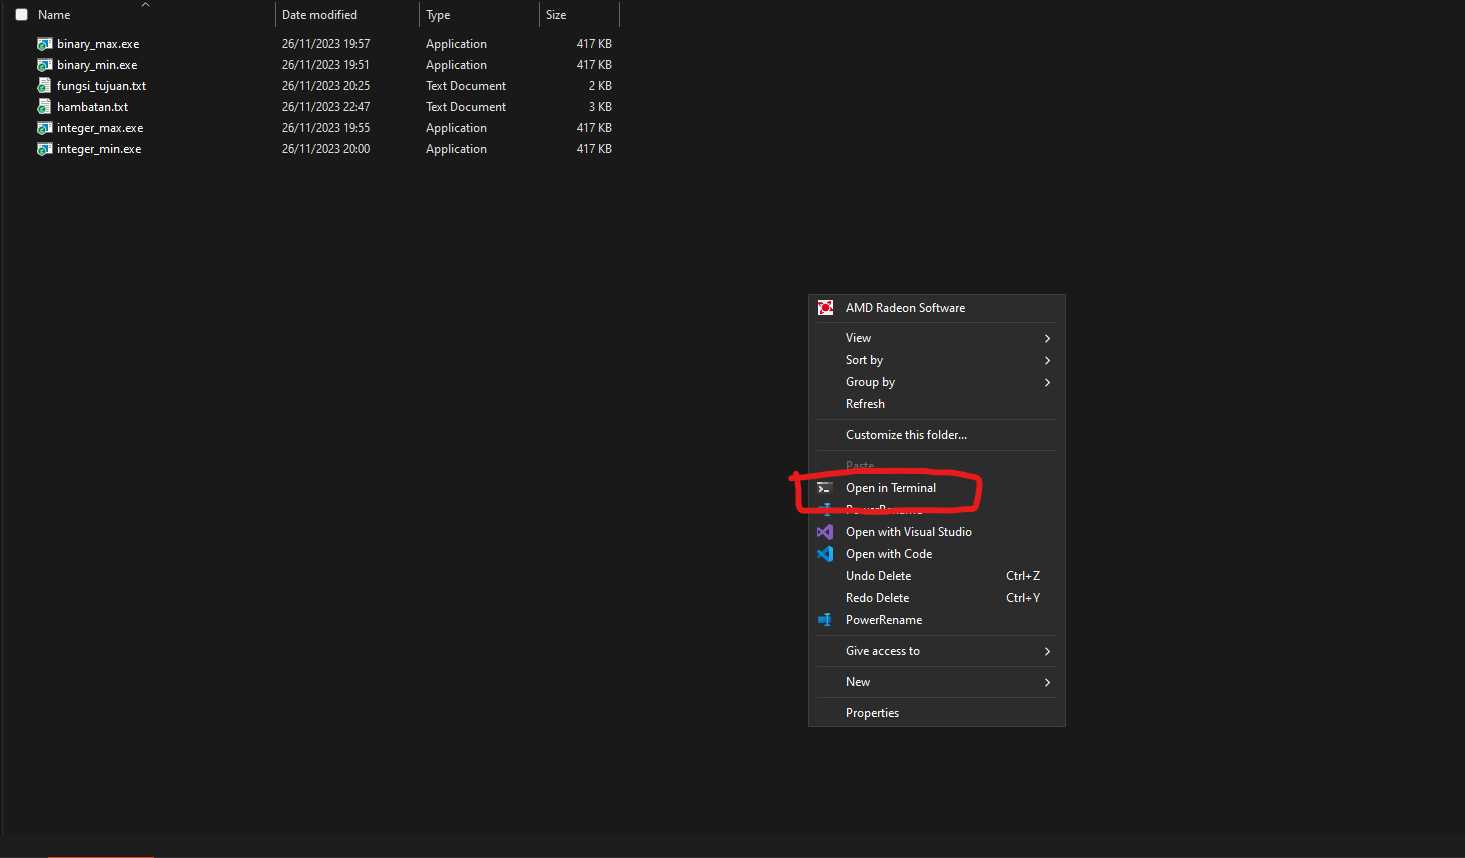
\includegraphics[scale=0.3]{1.png}
                \end{center}
            }\newpage
            \item {
                ketik \inline{.\\\{nama_exe\}.exe} lalu enter, jika muncul "\inline{Terjadi kesalahan}...", maka eror disebabkan kesalahan penulisan. Jika tidak, maka infeasible.
                \begin{center}
                    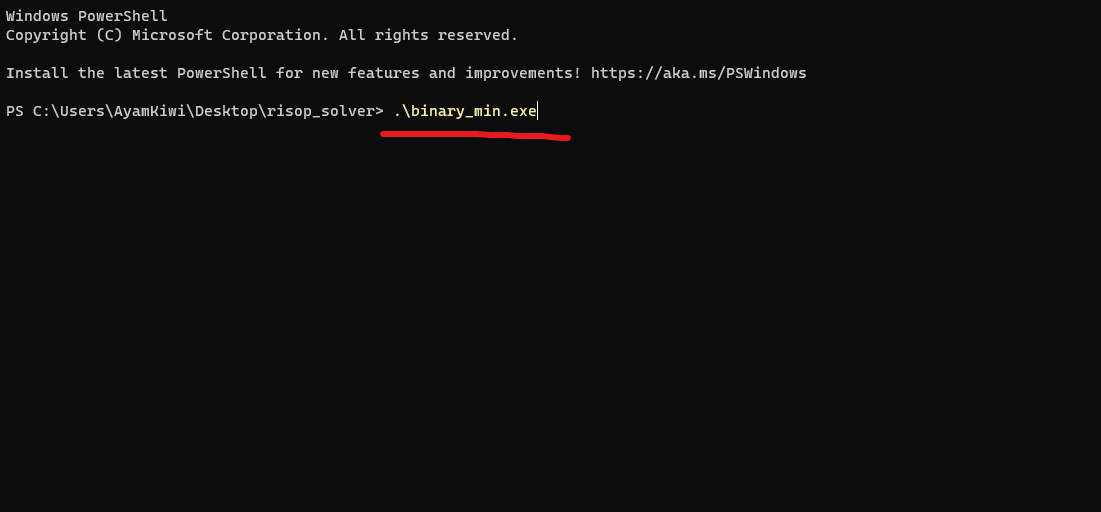
\includegraphics[scale=0.4]{2.png}
                \end{center}
            }
        \end{enumerate}
    }
\end{enumerate}
\vfil
\begin{center}
    
\includegraphics[]{hatsune_miku_24.png}
    
    goodluck

    \textcolor{gray}{note: mohon maklum jika banyak bug, error, atau hasilnya tidak sesuai ;))}
\end{center}
\end{document}